% Research plan
\chapter{Research plan}
\vspace{-1cm}

Four specific objectives were developed for this work, combining literature review, data analysis, analytical technique development, focused experimentation, and modeling:

\begin{itemize}
	\item Determine REE abundance and trends in natural waters.
	\item	Develop efficient liquid-liquid extraction technique for separation of REE from hypersaline brines
	\item Study the effects of ligand functionality and geometry on the partitioning behavior of the REE from brines to functionalized adsorbents
\end{itemize}

These individual tasks are described subsequently in \S 2.1–2.3.

\section{Determine REE abundance and trends in natural waters}

In this objective, a compilation and analysis of data from numerous independent studies of REE in natural waters was performed.
The compiled data were used to develop a consistent database of REE concentrations and their associated major solute chemistry and to explore interelement relationships, examine trends in REE abundance, and test hypotheses related to REE abundance as functions of major solution chemistry parameters.
The tasks within this objective were: (1) to ascertain an expected range of dissolved REE concentrations in waters of variable chemistries, (2) to derive unbiased estimates of REE distributions, and (3) to investigate trends in REE abundance in groundwater in relation to other available chemical parameters (e.g. pH, ionic strength, and major solution species).
Results of this work have been published and described in detail in \citet{Noack_EST_2014}.

The major findings of this work were that the REE are found in natural waters across ten orders of magnitude of concentrations, that pH appears to be the only variable at the ``macro'' scale of this study which significantly influences abundance, and that, while limited data exist for REE in brines, the REE composition of brines is potentially unique.
These results have implications on the remainder of this project.
First, the natural variability and lack of data of REE in brines necessitates development of robust, reliable analytical techniques for such waters as well as the application of this technique to hypersaline brine samples.
Second, the lack of consistent predictors of REE abundance requires focused experimentation of REE source and sink behavior in the environments of interest.

\section{Develop a liquid-liquid extraction technique for separation and concentration of REE from brines}

In this objective, REE separation and preconcentration from highly saline brines using a liquid-liquid method was studied.
A significant limitation of published methodologies for REE quantification in aqueous samples is the lack of validation of the methods in systems with high salinity and dissolved metals.
A common ligand used for REE complexation and extraction, bis(2-ethylhexyl) phosphate (HDEHP), was studied in a heptane diluent. 
The tasks of this objective were to: (1) demonstrate feasibility of REE recovery from small volumes of hypersaline brines by LLE, (2) optimize LLE methodology for high salinity and metals content, and (3) validate method for synthetic brines of varying complexity.
Results of this work have been published and described in detail in \citet{Noack_EST_2015}.

The major finding of this work was that the REE are measurable at environmentally relevant concentrations in hypersaline solutions with high accuracy using small volumes of samples.
Moreover, the method is robust to variability in salt, dissolved organic carbon, and competing metal concentrations.
This method can be confidently applied to the analysis of natural samples in the future for calibration of engineered recovery systems.

\section{Study REE partitioning to novel functionalized adsorbents from saline solutions}

In this objective, novel functionalized adsorbents were studied for the extraction and recovery of REE from geothermal fluids.
Geothermal fluids represent a promising alternative REE source given their known, elevated REE concentrations \citep{Michard_GCA_1989, Lewis_GCA_1997} and the large volumes in which they are handled daily ($\sim 100,000$ gal/MWe/day) \citep{CDOGGR}.
Extraction of the REE from these chemically complex fluids may be possible using high-capacity, REE-selective adsorbents in a fixed bed (or another configuration).
Experimentation and modeling as part of this objective will focus on the batch reactivities of two ligands known to have high REE affinity (phosphono-acetic acid, PAA, and Diethylenetriaminepentaacetic acid?, DTPA, which is grafted onto the surface as either an acid form or a dianhydride), which have been attached to an aminated silica gel support.
This work will be completed in collaboration with Kedar Perkins (Dept. Chem.) and Jon Callura (CEE), and will serve as the basis for an ongoing study of REE extraction from geothermal fluids.

\subsection{Material characterization}

A key component of understanding the reactivities of our adsorbents is the thorough characterization of the materials.
Multiple techniques will be used to characterize the functionalized adsorbents including thermogravimetric analysis (TGA), acid-base titrations, electrophoretic mobility measurements, and X-ray photoelectron spectroscopy.
Figure~\ref{fig:TGA-comb} illustrates the results of TGA for the unfunctionalized, 3-aminopropyl silica gel (AP-SiO2) as well as the DTPA-functionalized resin.
For each sample, the concentration of sites was detemined to be 1 mmol/g, which agrees with the specification provided by the AP-SiO2 manufacturer.
Figure~\ref{fig:titr} illustrates the conversion of the basic surface amines of the unfunctionalized material to an acidic form as a result of the functionalization scheme (addition of carboxyl groups).

\begin{figure}[htbp]
\begin{center}
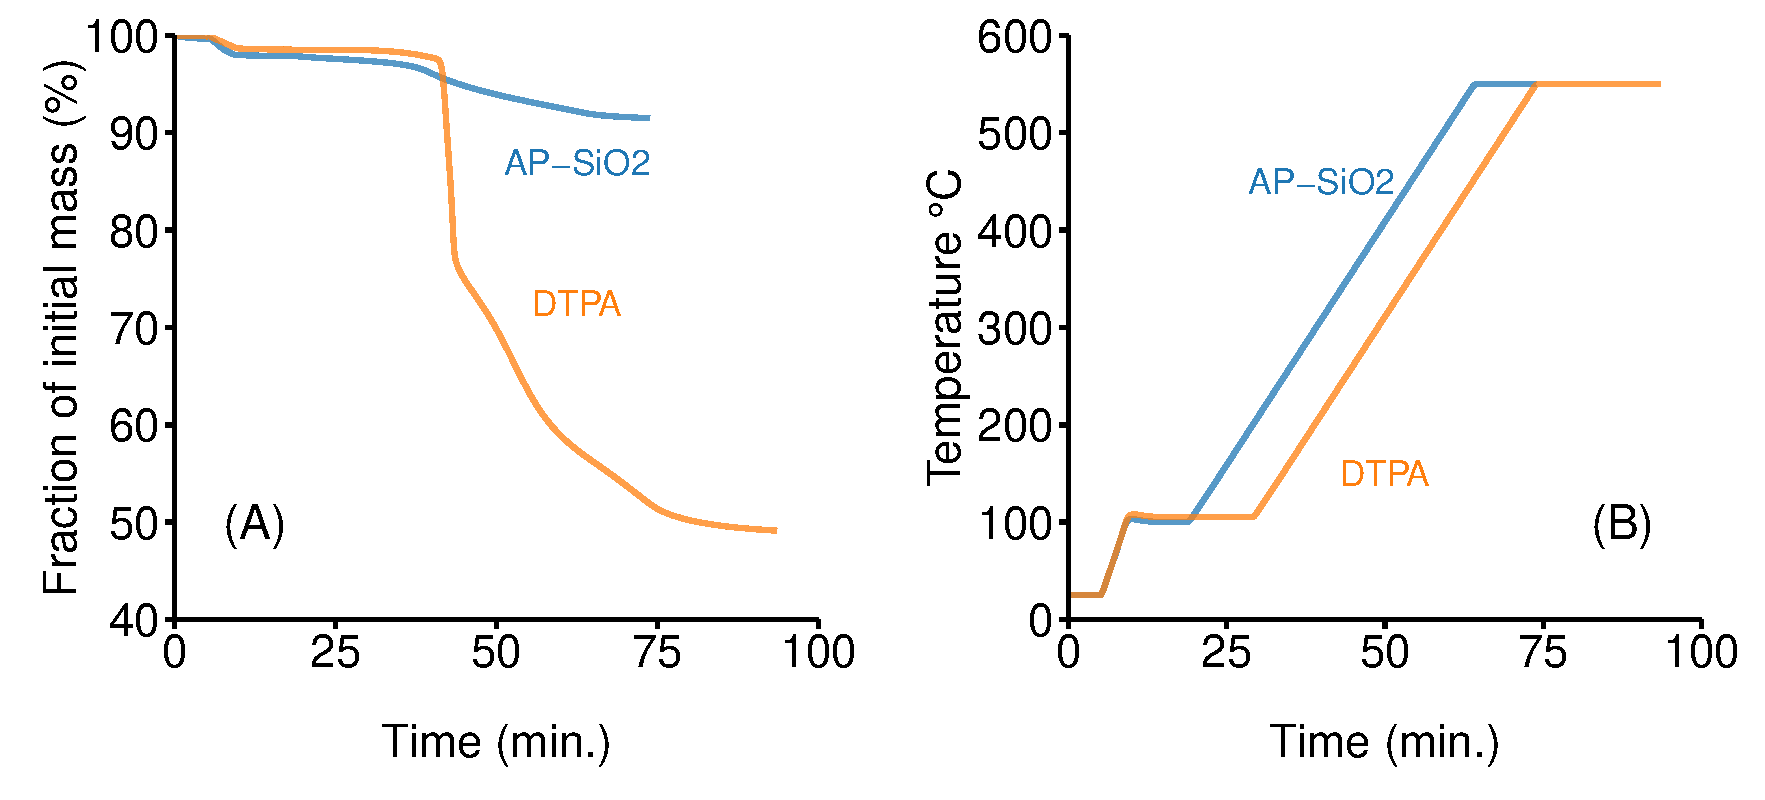
\includegraphics[width = \textwidth]{proposal_figures/DTPA-raw-TGA-combined.pdf}
\caption{Thermogravimetric analysis (TGA) of starting material (AP-SiO2) and DTPA-functionalized adsorbent. (A) Mass loss vs. time for two solids tested. Using the molecular weights of each surface group, the site concentration is calculated to be 1 mmol/g for each solid. (B) Temperature ramp programs used for TGA.}\label{fig:TGA-comb}
\end{center}
\end{figure}

\begin{figure}[htbp]
\begin{center}
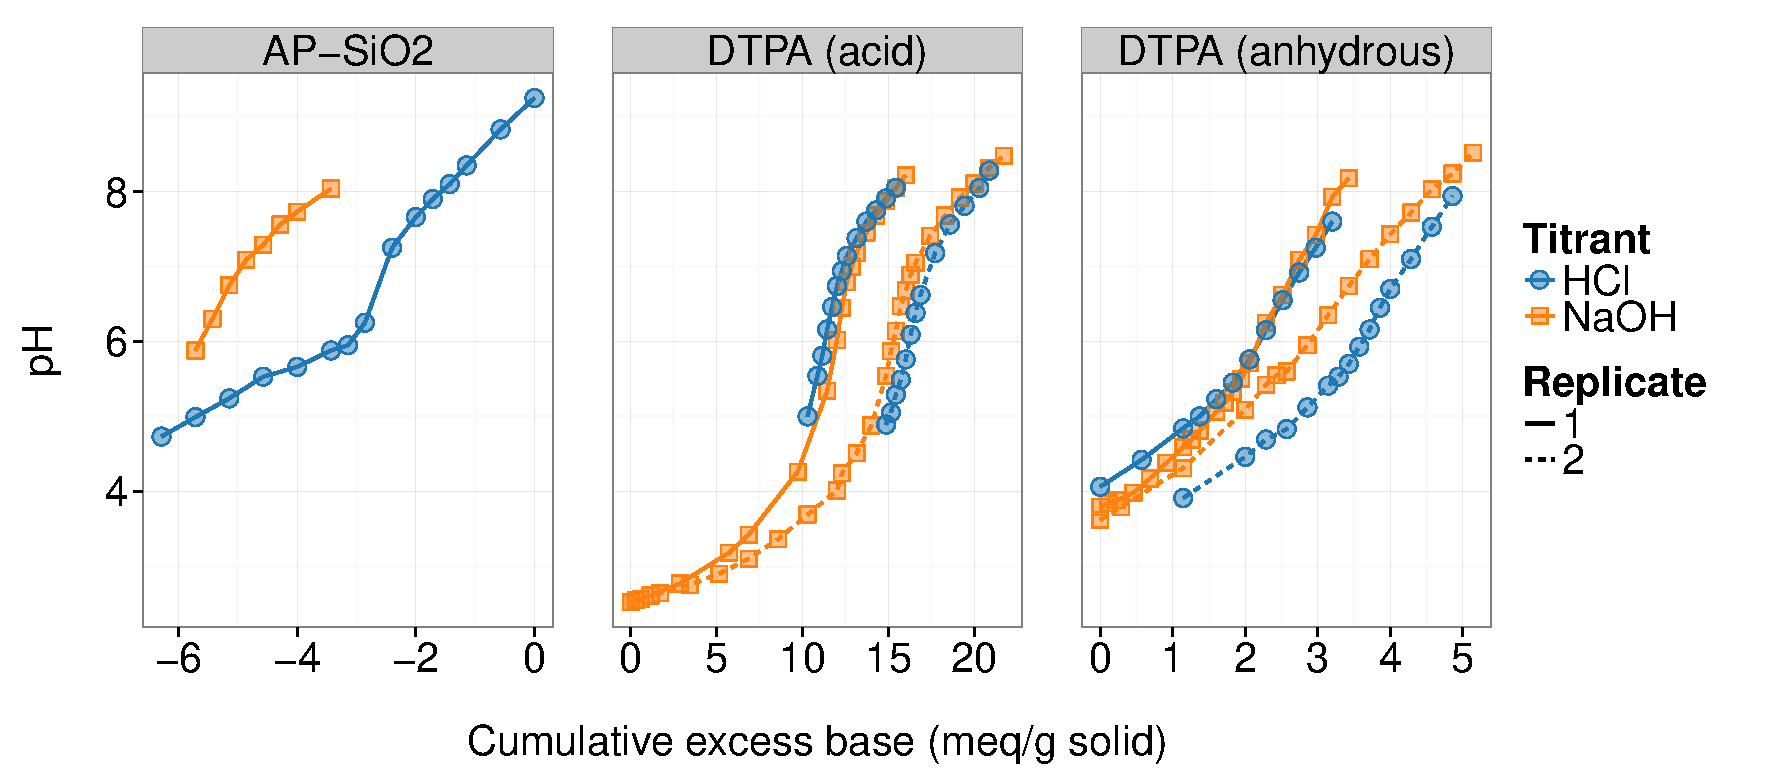
\includegraphics[width = \textwidth]{proposal_figures/Titrations.pdf}
\caption{Titration curves for the raw, un-functionalized support (3-aminopropyl silica gel, 3-AP Si) and for two forms of the functionalized resins (DTPA (acid) and DTPA (anhydrous)).
Titrations were performed in 5 g solid L$^{-1}$ suspensions in a 0.5 M NaCl electrolyte.
Solid and dotted lines indicate replicate titrations.
Note that the x-axes for each panel are unequal while the y-axes are uniform.}\label{fig:titr}
\end{center}
\end{figure}

\subsection{Adsorption edges}

Adsorption edges will be used to study the pH dependency of the adsorbent performance.
Some preliminary data for anhydrous-DTPA is shown for 0.5 M and 3.0 M NaCl using Nd, Gd, and Ho as characteristic REE in Figure~\ref{fig:ads-edge-ionic-strength}.
From these results, we see peculiar behavior where the REE are bound significantly at low pH, but do not adsorb at mid-range/circum neutral pH as would be expected based on carboxyl-functionality (``expected'' model behavior for DTPA shown in Figure~\ref{fig:DTPA-model}).
Additional testing is underway to determine the sources of this deviation.
Adsorption edges will be generated for all functionalized materials (PAA and both DTPA forms).

\begin{figure}[htbp]
\begin{center}
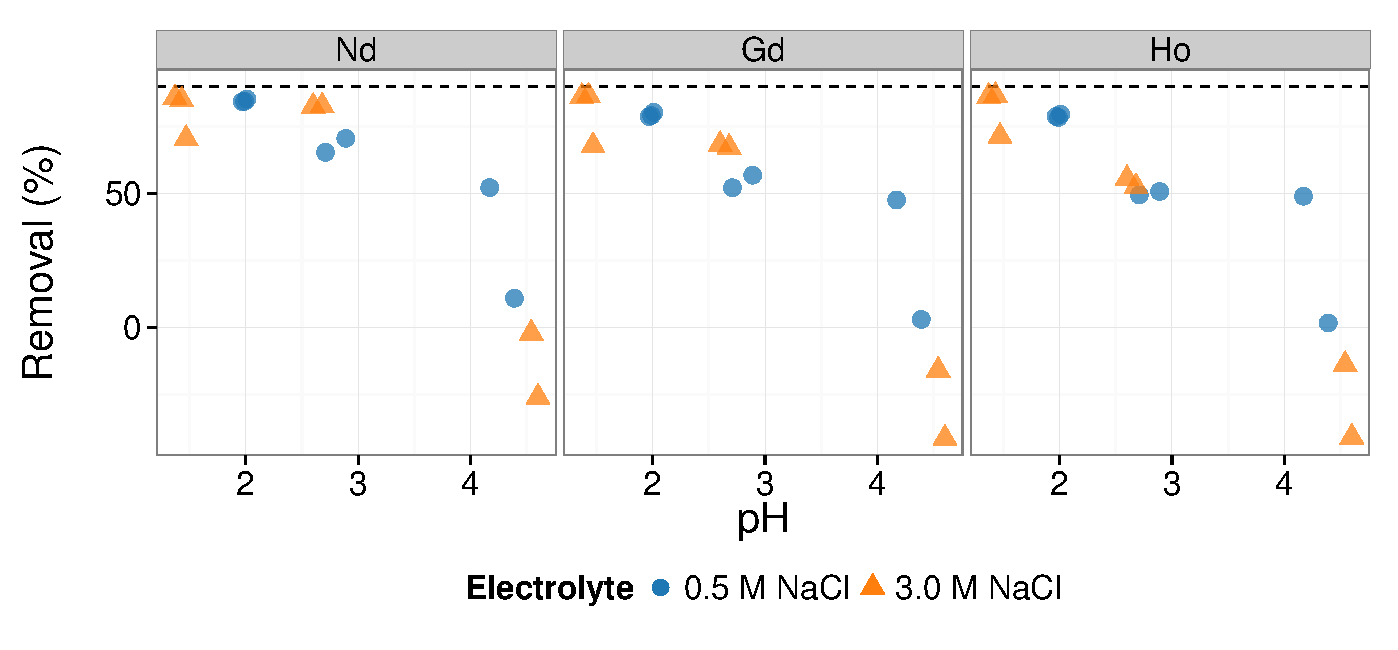
\includegraphics[width = \textwidth]{proposal_figures/ionic-strength-effects_2015-10-13.pdf}
\caption{REE removal ($1 - C_f/C_i$; $C_i = 100$ ppb each REE) from saline solutions as a function of pH for two different electrolyte concentrations using 10 g/L anhydrous-DTPA functionalized silica gels.
Contact time was 3 hours.
Dashed line indicates 90\% removal.
Large negative removals shown are likely a result of pipette error when diluting 3 M NaCl samples for analysis, but based on reagent purities (no detectable REE contamination) these can be effectively be treated as zero.}\label{fig:ads-edge-ionic-strength}
\end{center}
\end{figure}

\begin{figure}[htbp]
\begin{center}
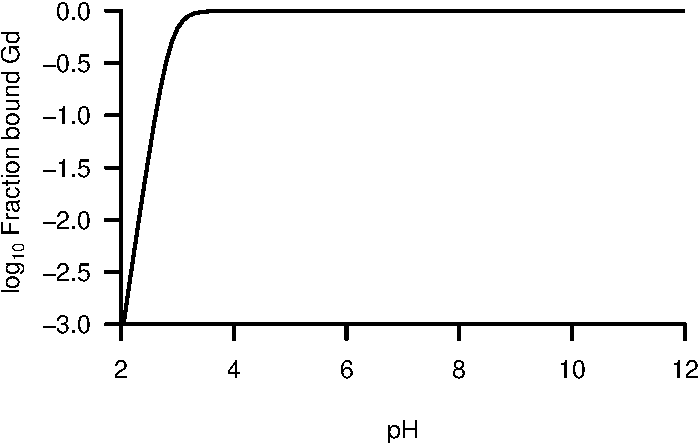
\includegraphics[width = 0.6\textwidth]{proposal_figures/DTPA-binding-model.pdf}
\caption{Predicted adsorption isotherm for DTPA-functionalized resin, using aqueous thermodynamic data in lieu of a surface complexation model.
Model considered the following species of Gd: \ce{Gd^3+}, \ce{GdOH^2+}, \ce{Gd(OH)2+}, \ce{Gd(OH)3^0}, \ce{GdCl^2+}, \ce{Gd(DTPA)^2-}, and \ce{Gd(HDTPA)-}.
Association constants for these species are taken from \citet{Lee_GCA_1992} for the hydrolysis products, \citet{Millero_GCA_1992} for the chloride complex, and \citet{Grimes_JSC_2014} for the DTPA species (which also include the acid-dissociation constants for DTPA).
Calculation conditions were [Gd]$_{tot}=$ 100 ppb, [DTPA]$_{tot}=$ 10 mM, 0.5 M NaCl.}\label{fig:DTPA-model}
\end{center}
\end{figure}

\subsection{Uptake kinetics}

The surface complexation/adsorption kinetics of these adsorbents is a critical design parameter for fixed bed deployment.
These uptake kinetics will be studied in batch for all adsorbents.
Figure~\ref{fig:ads-edge-kinetics} illustrates that not only are there kinetic limitations to the adsorption (evidenced by the significant increase from 3 hours to 3 days of contact time), but that it is also element dependent, potentially based on ionic size ($r_{3+}$: Nd$>$Gd$>$Ho) as the thermodynamic affinities display a reverse trend \citep{Grimes_JSC_2014}.
Kinetic tests will utilize higher REE concentrations, so that small aliquots can be removed from each reactor and diluted for measurement without significantly altering the solid-liquid ratio.
Because reactor pH cannot be measured \textit{in situ}, it will only be recorded before REE addition and at the end of contact time.
Suspensions will be pre-equilibrated with appropriate acid or base doses prior to REE dosing to minimize pH changes during reaction.

\begin{figure}[htbp]
\begin{center}
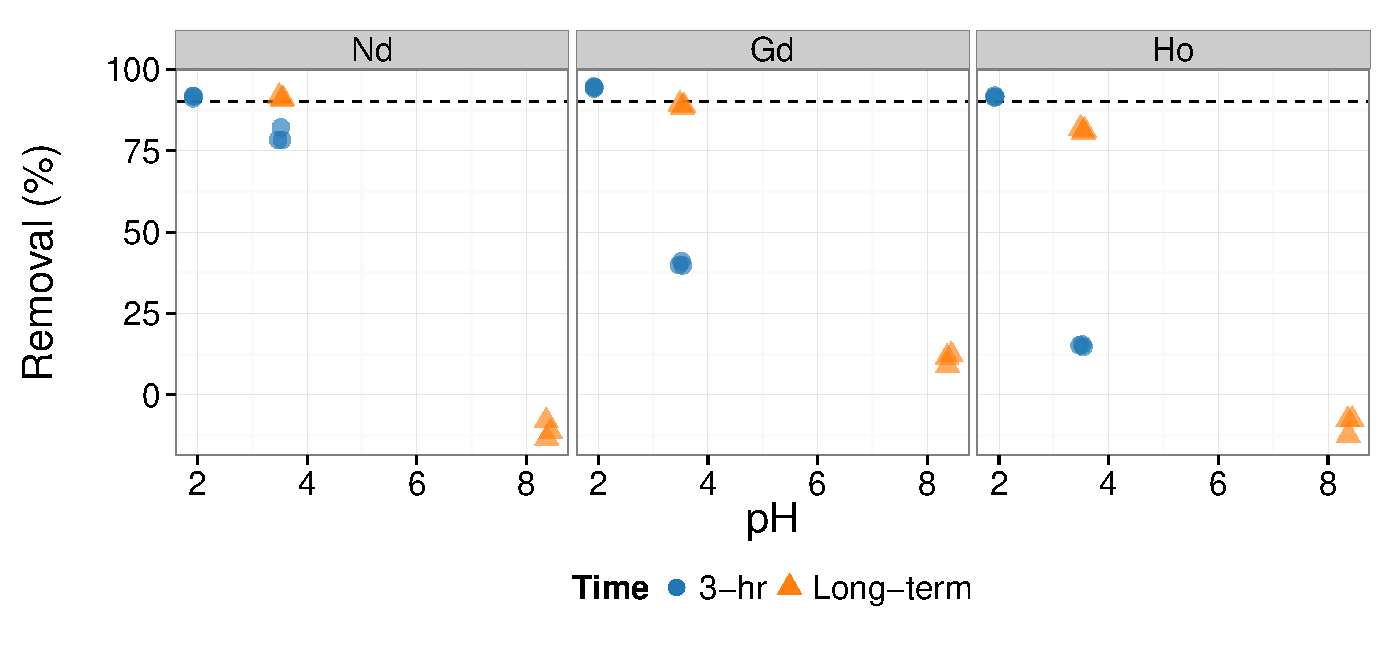
\includegraphics[width = \textwidth]{proposal_figures/pseudo-eq-ads_2015-09-23.pdf}
\caption{REE removal ($1 - C_f/C_i$; $C_i = 100$ ppb each REE) from 0.5 M NaCl as a function of pH for two different contact times using 10 g/L anhydrous-DTPA functionalized silica gels.
Contact times were 3 hours and 3 days.
Dashed line indicates 90\% removal.}\label{fig:ads-edge-kinetics}
\end{center}
\end{figure}

\subsection{Constant pH isotherms}

Constant pH isotherms will provide useful data regarding the REE affinity ($K_{LF}$) of the functionalized materials as well as the effective capacity ($q_{max}$).
\citet{Roosen_JMC_2014} functionalized a silica--chitosan hybrid support with DTPA and found that the isotherm data were well fit by a Langmuir-Freundlich model (Eq.~\ref{eq:LF-eq}).

\begin{equation}\label{eq:LF-eq}
q_e = q_{max} \left( \frac{(K_{LF}C_e)^n}{1 + (K_{LF}C_e)^n} \right)
\end{equation}

Solid suspensions, pre-equilibrated with acid or bases doses, will be mixed with varied REE doses for a contact time determined from kinetic experiments.

\subsection{Tests of REE-selectivity}

In the complex aqueous systems of interest, the REE will compose a trace component of the bulk solutes.
Therefore, it is important to understand the effects of competitive cations on REE uptake by our functionalized materials.
Based on atomic radii, calcium (which is abundant in geothermal fluids) may be a potent competitor given the large mass action advantage of higher concentration.
Figure~\ref{fig:Ca-comp} shows that for a $3:1$ Ca:Gd ratio, no significant decrease of Gd adsorption is observed.
Future competition tests will focus on more relevant solute concentrations, determined based on literature review of geothermal fluids \citep[e.g.][]{ProdWat}, as well as other metals.

\begin{figure}[htbp]
\begin{center}
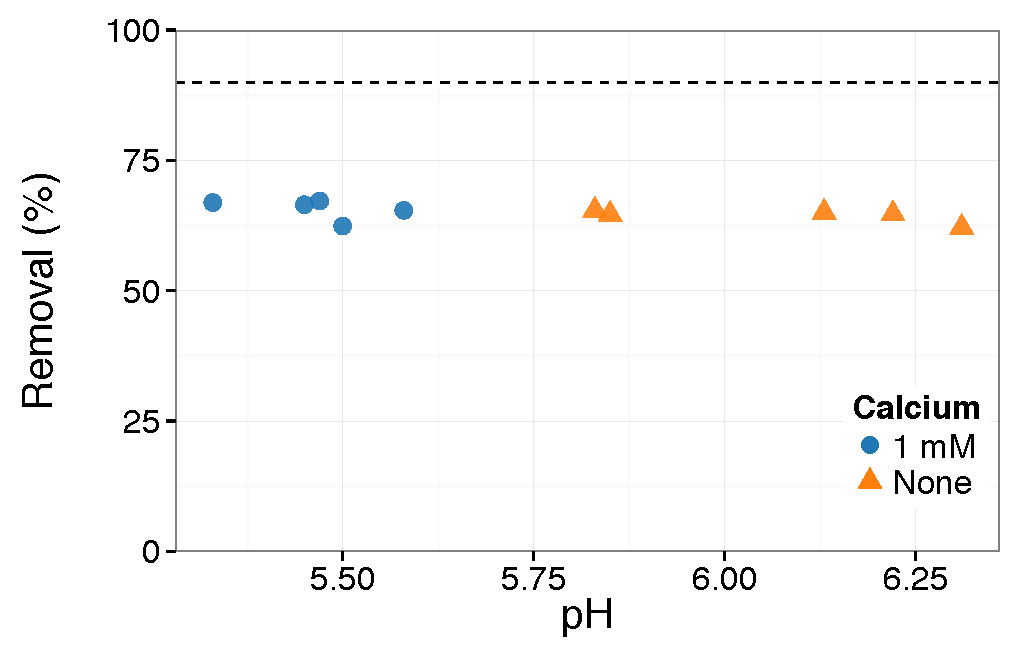
\includegraphics[width = 0.7\textwidth]{proposal_figures/DTPAa-Ca-comp.pdf}
\caption{Gd removal ($1 - C_f/C_i$; $Ci = 300$ \si{\micro}M Gd) from 0.5 M NaCl solutions as a function of pH with and without Ca dosing using 10 g/L anhydrous-DTPA functionalized silica gels.
Contact time was 3 hours.
Dashed line indicates 90\% removal. }\label{fig:Ca-comp}
\end{center}
\end{figure}
